\setAuthor{Richard Luhtaru}
\setRound{piirkonnavoor}
\setYear{2022}
\setNumber{G 1}
\setDifficulty{1}
\setTopic{TODO}

\prob{Peegel peeglis}
Toas on kaks tasapeeglit. Arvo (tähistatud punktiga $A$) nägi peeglisse vaadates Pärti (tähistatud punktiga $B$). Konstrueerige kiirte käik, kuidas Arvo võis peegli(te) abil Pärti näha. Leidke kõik võimalused. Lahendage ülesanne lisalehel.
\begin{figure}[h]
  \vspace{-1em}
  \centering
  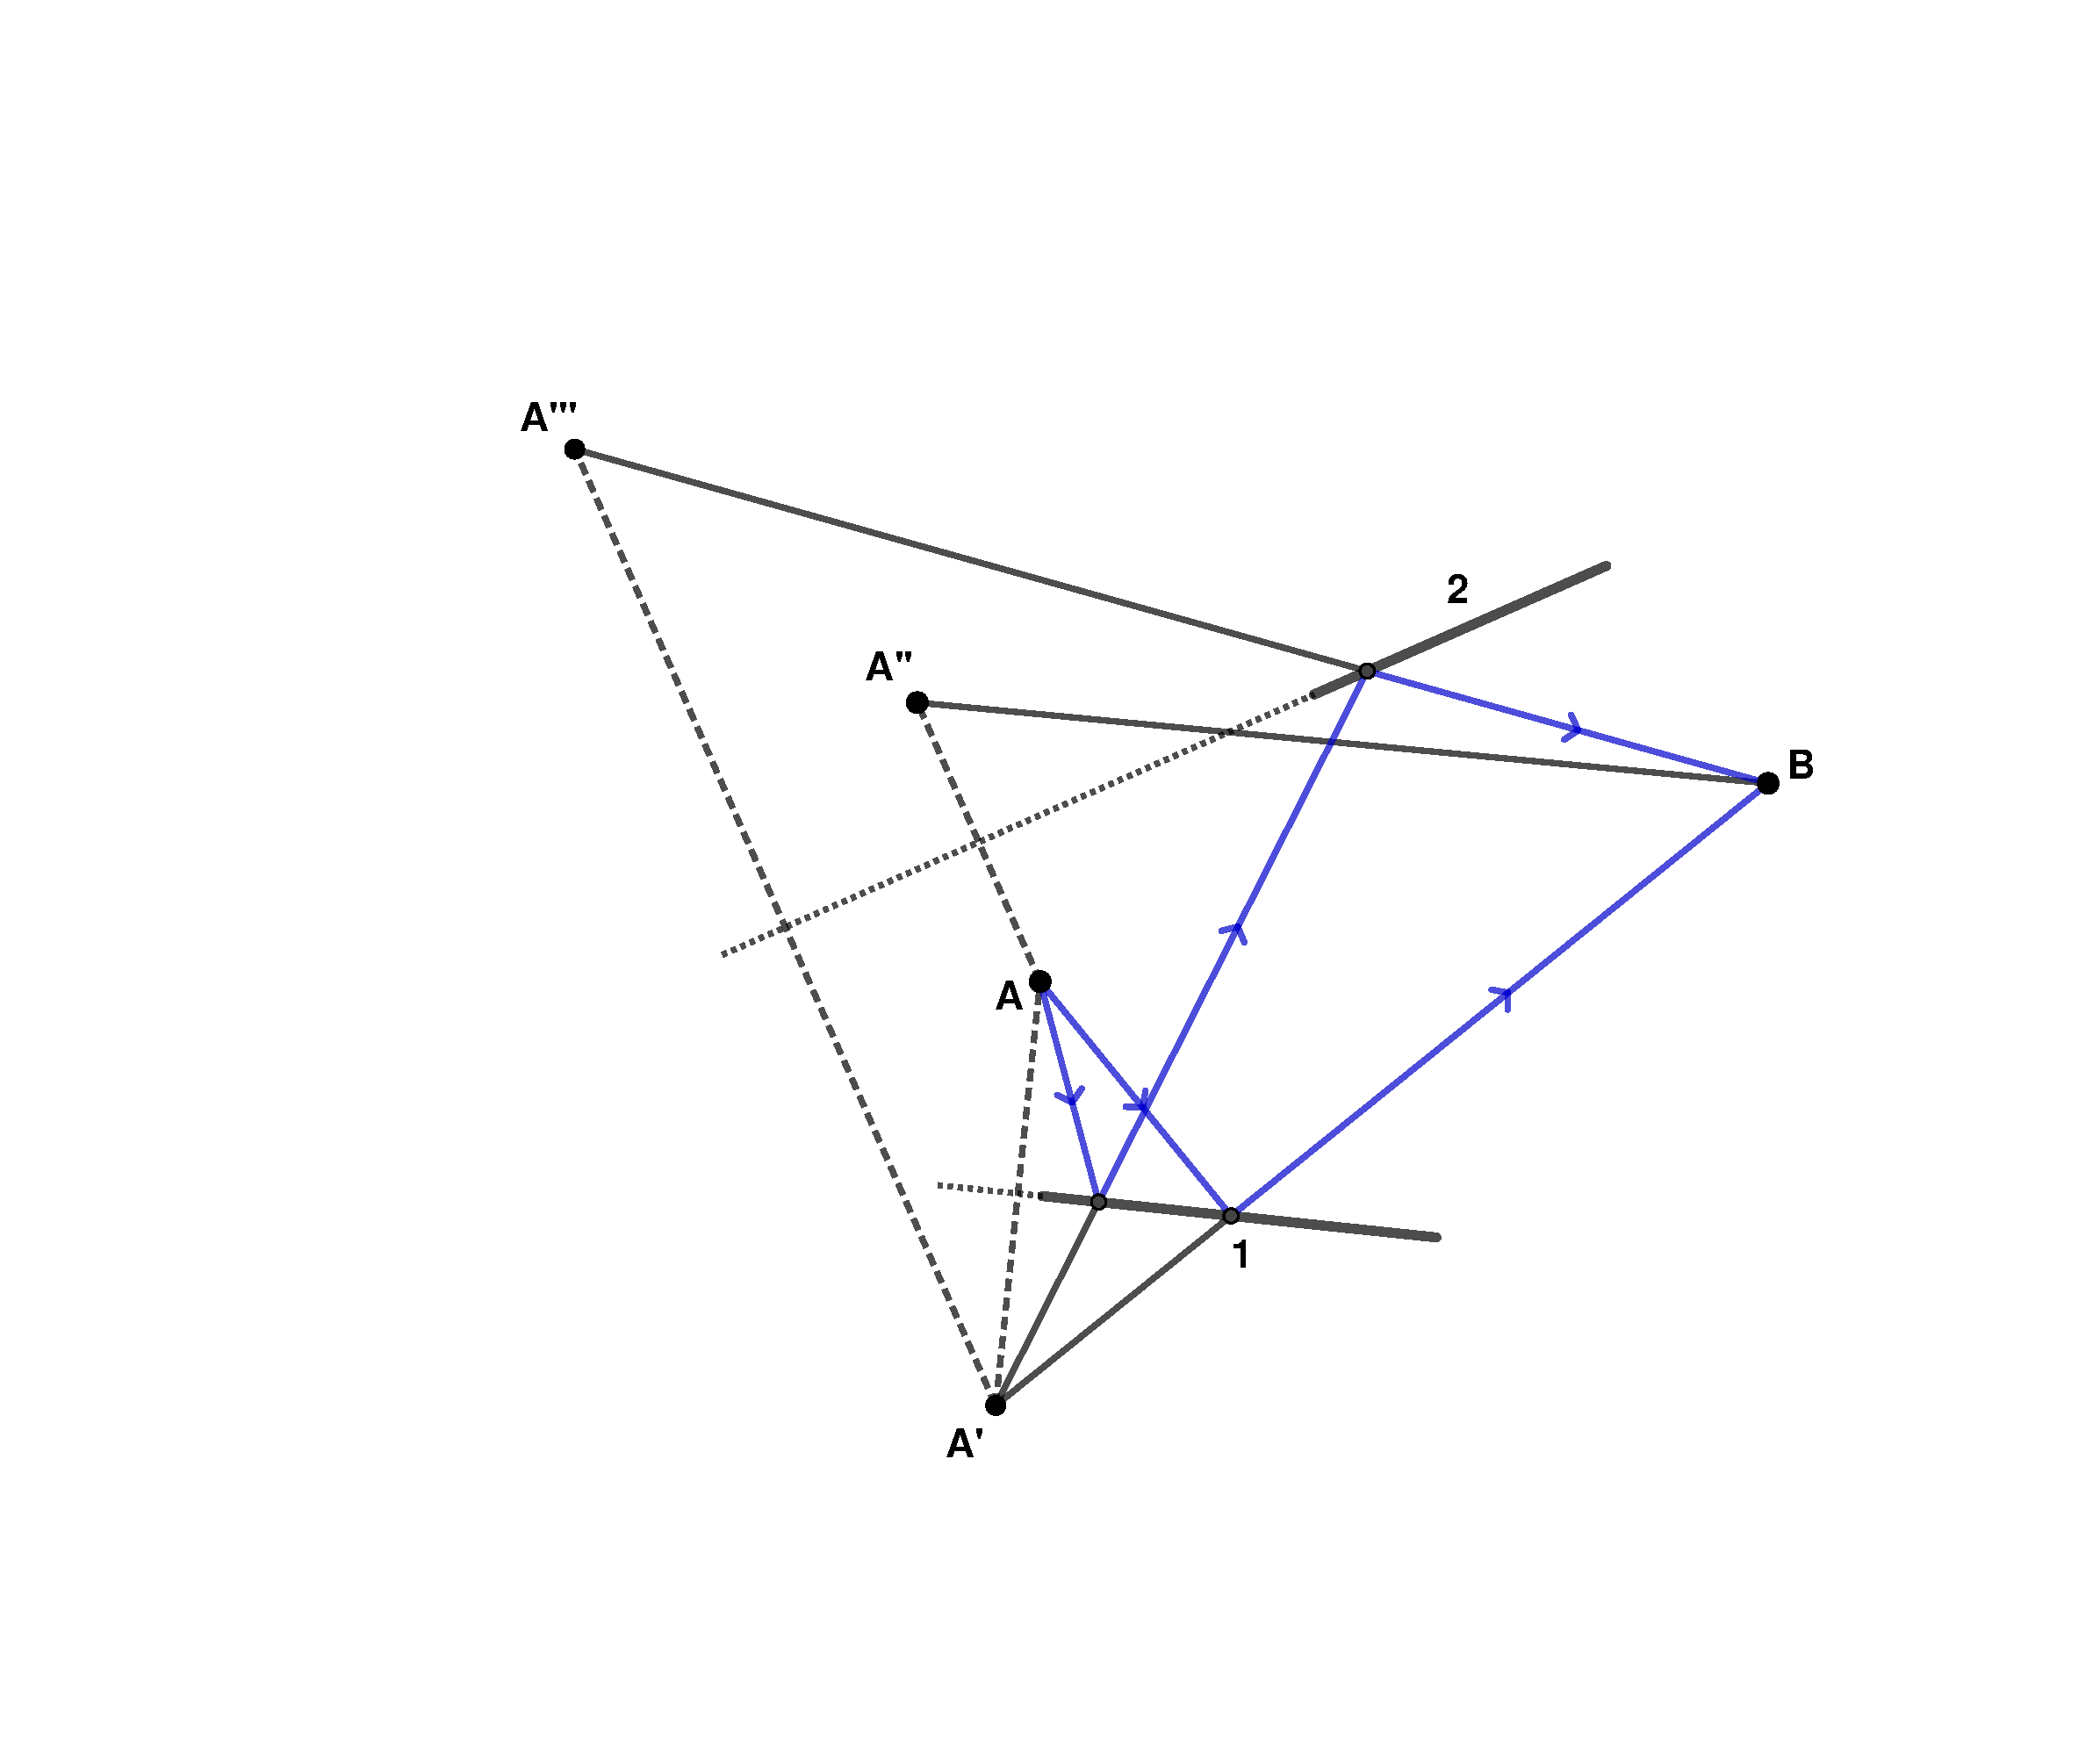
\includegraphics[height=11em, trim=0 80 0 140, clip]{2022-v2g-01-yl.pdf}
  \vspace{-2em}
\end{figure}


\hint

\solu
Konstrueerime Arvo kujutise peeglis 1 ($A'$), peeglis 2 ($A''$) ja punkti $A'$ kujutise peeglis 2 ($A'''$). Breti nägemiseks on kaks võimalust. Esimene võimalus on ainult peegli 1 kaudu, kiirte käigu saame konstrueerida lõigu $A'B$ abil. Teine võimalus on peegli 1 ja seejärel peegli 2 kaudu, kiirte käigu saame konstrueerida lõigu $A'''B$ abil. Ainult peeglist 2 pole võimalik Bretti näha, sest $A''B$ ei lõiku peegliga 2. Samuti pole peeglist 2 võimalik näha peeglit 1, seega rohkem võimalusi pole.

\begin{figure}[h]
    \centering
    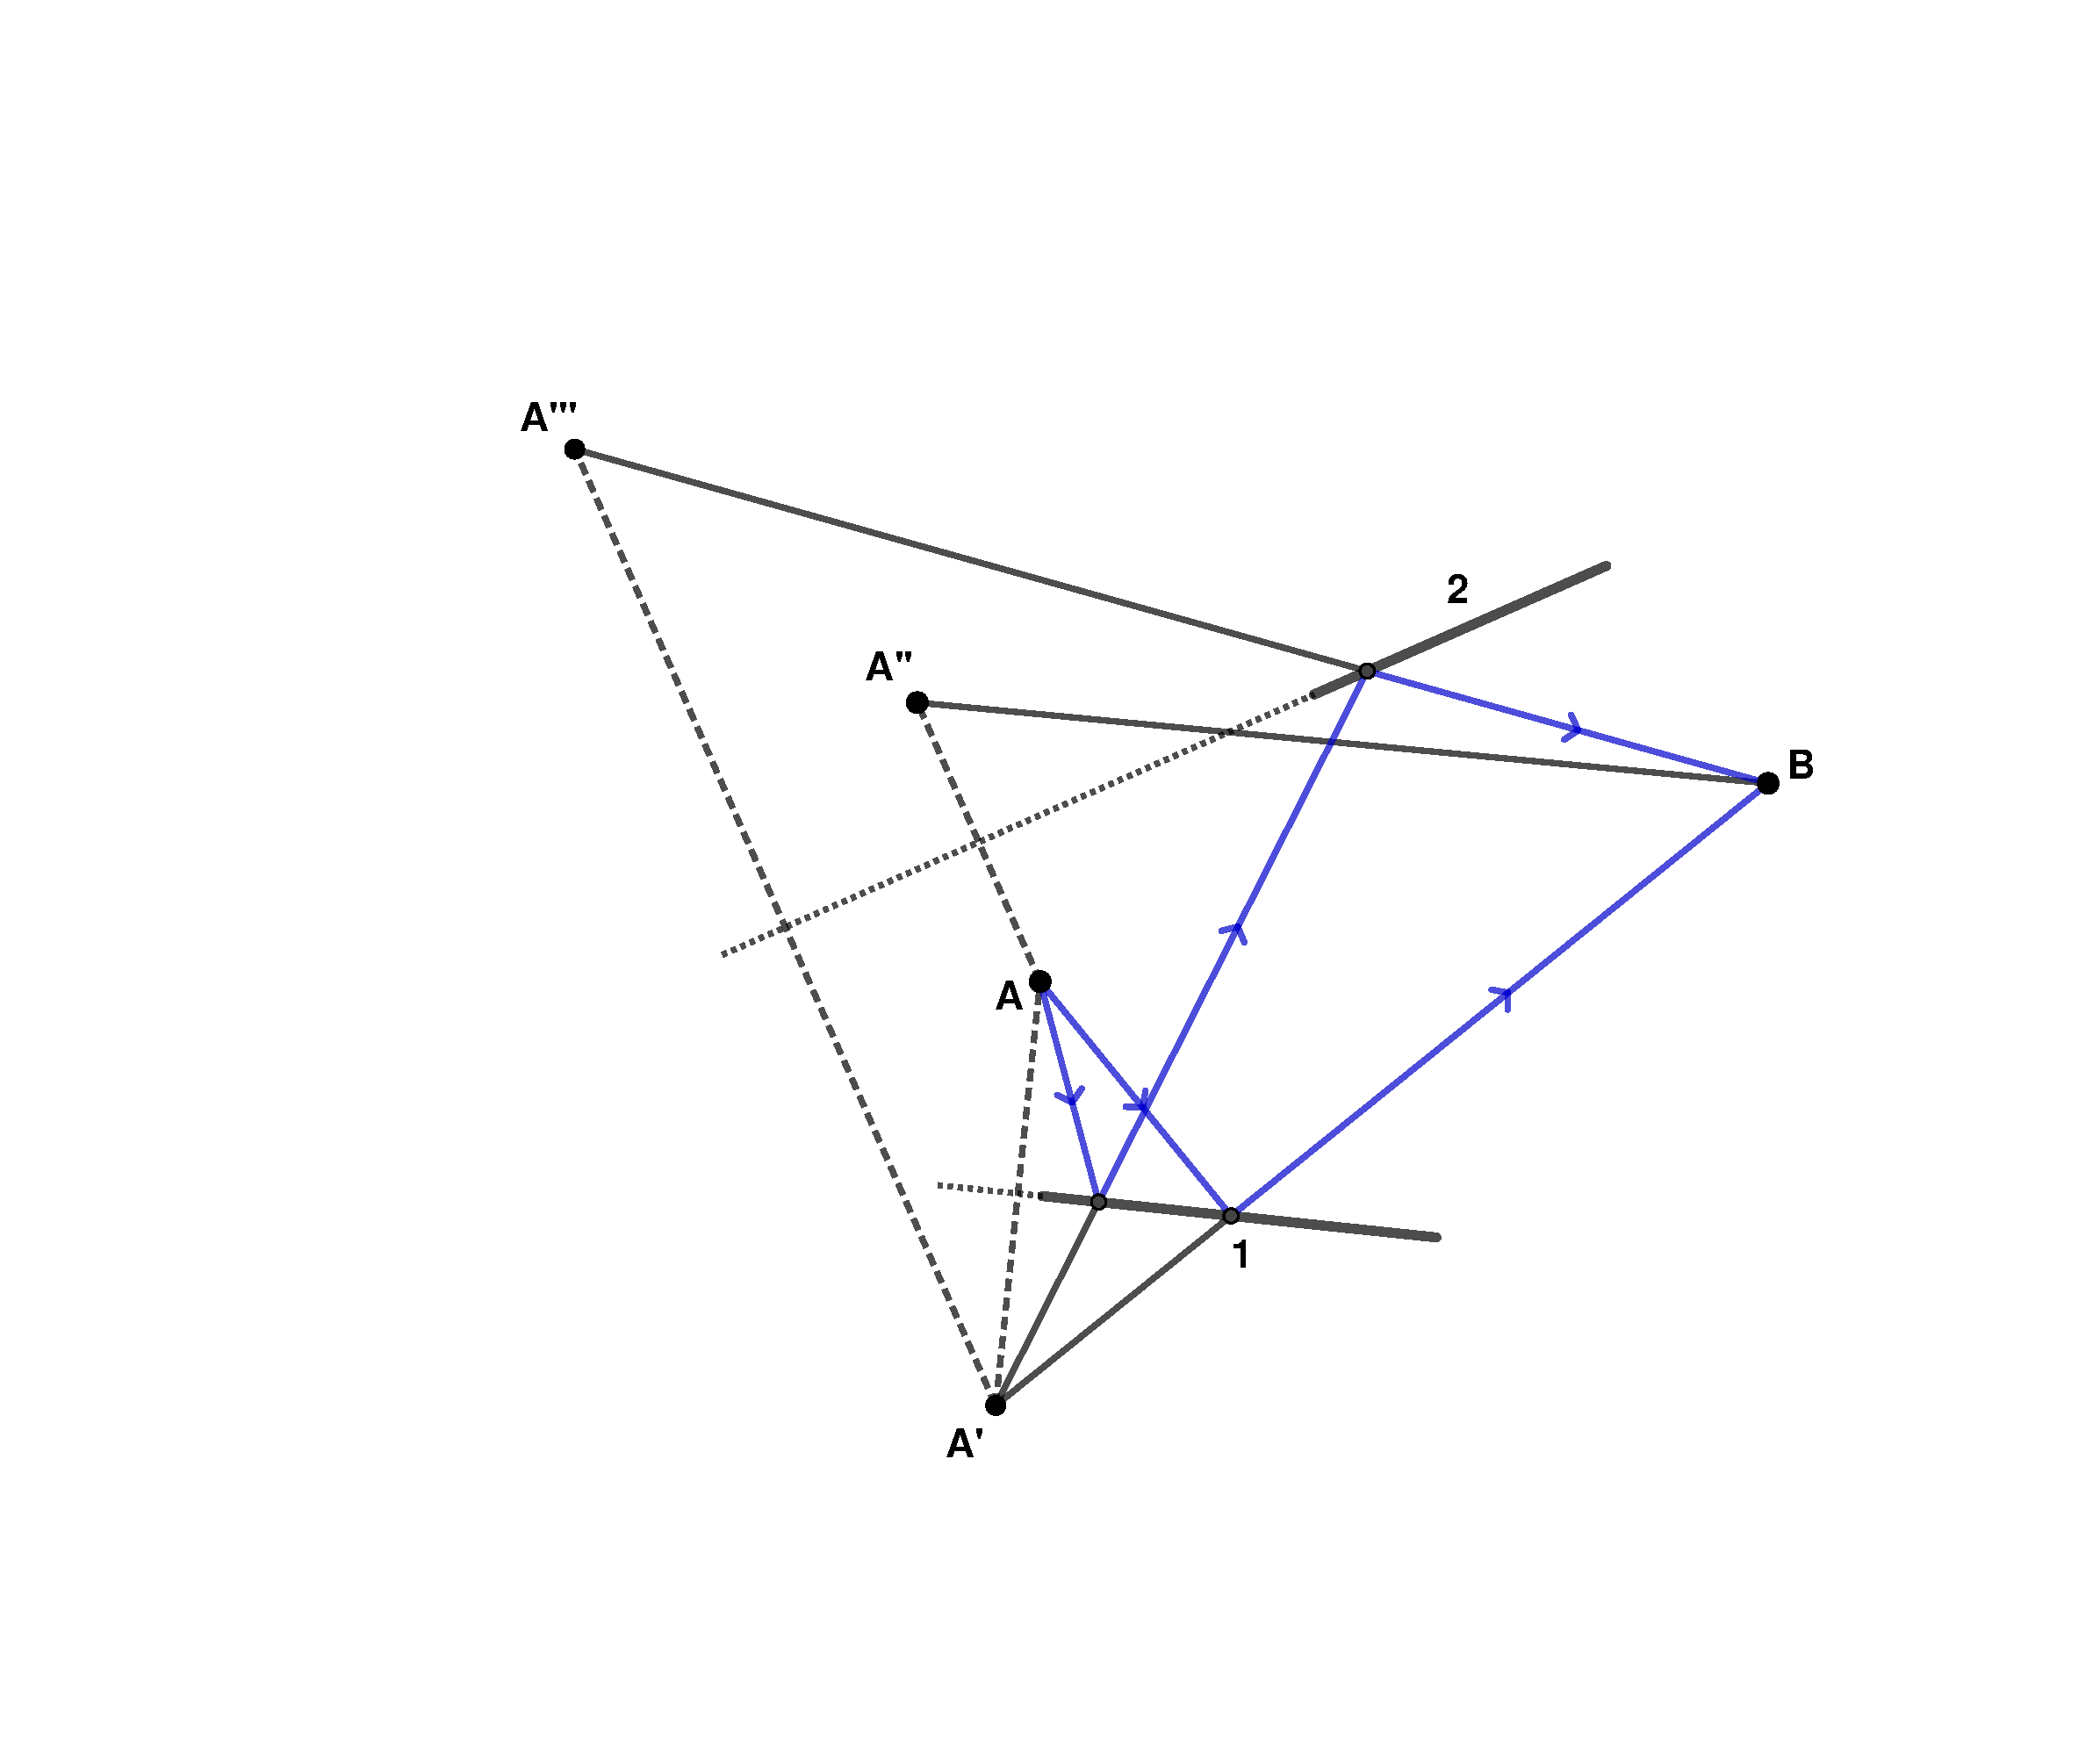
\includegraphics[width=\textwidth, trim=0 50 0 50, clip]{2022-v2g-01-yl.pdf}
\end{figure}
\probend